%!TEX root = ../Thesis.tex

\section{GUI-Konzept \textcolor{blue}{[Julius Figge]}}

Wir haben uns entschieden, statt eines GUI-Mockups unser GUI-Konzept direkt im Prototypen mit auszuliefern.
Das lässt sich durch mehrere Punkte begründen.
Zuerst hatten wir zum Zeitpunkt der ersten Präsentation bereits einen funktionierenden Prototypen und konnten diesen direkt mit dem GUI-Konzept ausstatten. Dadurch hatten wir nicht nur ein Mockup sondern konnten bereits mit der GUI interagieren.
Des weiteren hatten wir dadurch die Möglichkeit die Zeit für die Erstellung eines Konzeptes direkt in die Entwicklung funktionierender GUI zu stecken.

Die GUI wurde unter Nutzung von Bootstrap 4 in Kombination mit Font-Awesome für die Icons entwickelt. 
Dadurch war es uns mögliche eine konsistente, verständliche und klare Oberfläche zu entwickeln.
Hierbei haben wir uns darauf konzentriert \enquote{eine klare Linie zu fahren}. Alle Seiten werden auf weißem Hintergrund dargestellt. Buttons und Informationen sind generell in grau ( beziehungsweise Schwarz) gehalten. 
Abweichend hiervon treten Farben nur auf um die Aufmerksamkeit des Nutzers auf sich zu ziehen oder um Hinweise hervorzuheben. Diese Farben sind in \cref{fig:Farbmuster} abgebildet. Die Verwendung wird im weiteren näher erläutert.

\begin{figure}[hbt]
\centering
\begin{minipage}[t]{1\textwidth}
    \caption{Farben Konzept}
    \includegraphics[width=0.5\textwidth]{img/Farbmuster.png}\\
    \source{Eigene Darstellung}
    \label{fig:farbmuster}
\end{minipage}
\end{figure}


Grundlegend sind die Elemente der Anwendung zentriert wie im weiteren zu sehen. Damit erreichen wir in Kombination mit der Nutzung von Bootstrap eine nahezu 100 prozentige Kompatibilität zu mobilen Endgeräten.\footnote{Hierbei ist jedoch anzumerken, dass dieses Feature nicht gefordert war und somit auch nicht weitergehend getestet wurde. Allerdings sind bereits die Voraussetzungen für eine mögliche Erweiterung der Anwendung geschaffen.}

Grundlegende Elemente dieses Konzeptes sind zum einen der Login-Screen (Siehe \cref{fig:Login} im Anhang auf S.\pageref{fig:Login}).
In diesem Screenshot ist auch das Logo der Anwendung zu sehen welches ebenfalls in den typischen Farben gehalten wurde. Dieses soll der Anwendung einen Wiedererkennungswert geben durch seine gleichzeitig humorvolle als auch simple Darstellung.

Die zweite zentrale Komponente des Konzeptes ist die Übersicht aller Ideen (Siehe \cref{fig:ideen}).
Auffallend ist hier die Gliederung der Ideen in Tabellen. Bereits zu diesem Zeitpunkt war geplant die Ideen nach Typ zu gliedern und in einer Übersicht mit ihren wichtigsten Eigenschaften darzustellen. 
Zu diesem Zeitpunkt noch per Klick\footnote{Diese Funktionalität wurde im weiteren durch ein Rechtsklick Menü erweitert (Siehe \ref{GUI-Umsetzung} S.\pageref{GUI-Umsetzung}).}, sollte es möglich sein die Idee im Detail inklusive aller Informationen darzustellen. Diese Entscheidung begründest sich damit das Gleichgewicht zwischen der verfügbaren Information auf einer Seitenansicht und der Übersichtlichkeit zu wahren.
Darüber hinaus findet sich auch hier die Farbgestaltung wieder. Grundsätzlich ist die Oberfläche Monochrom gehalten. Icons dienen der schnelleren Identifikation der verschiedenen Tabellen und der Übersichtlichkeit. Farbakzente sind zum einen zur Führung der Nutzer gedacht, siehe beispielhaft in dem Hyperlink auf den Ersteller der Ideen\footnote{Dieser Hyperlink stand beispielhaft für die Weiterleitung auf eine Detailseite auf der Tabellensicht.}. Zum anderen sind diese in den Status der Ideen mit einbezogen, hierdurch lässt sich erheblich schneller ein Überblick verschaffen.

\begin{figure}[hbt]
\centering
\begin{minipage}[t]{1\textwidth}
    \caption{Ideen Konzept}
    \includegraphics[width=1\textwidth]{img/ideen-Konzept.png}\\
    \source{Eigene Darstellung}
    \label{fig:ideen}
\end{minipage}
\end{figure}

Ein weiterer relevanter Punkt der sich beispielhaft in dieser Abbildung (Siehe \cref{fig:ideen}) findet ist die Navigationsleiste. Diese ist im Konzept nur nach dem Login vorhanden. Im fertigen Produkt wurde diese aber auf jeder Seite inkludiert.\footnote{Ebenso wurde ein Footer eingefügt. Vgl. \ref{GUI-Umsetzung} S.\pageref{GUI-Umsetzung}}
Diese ist zentrales Steuerelement der Anwendung. Auf der linken Seite findet sich das Logo dauerhaft präsent wieder. Daneben werden zur Verfügung stehende Seiten angezeigt, wobei die aktuelle hervorgehoben ist.\footnote{Im fertigen Produkt ist diese Sicht abhängig von den verschiedenen Rollen. Vgl. \ref{GUI-Umsetzung} S.\pageref{GUI-Umsetzung}} Auf der rechten Seite findet sich der Logout Button, auch dieser ist hervorgehoben um vom Nutzer wahrgenommen zu werden.

Die weiteren Konzeptteile der GUI finden sich im Anhang \ref{GUI-Konzept} auf S.\pageref{GUI-Konzept}.

\begin{figure}[hbt]
\centering
\begin{minipage}[t]{1\textwidth}
    \caption{Rechtsklick Umsetzung}
    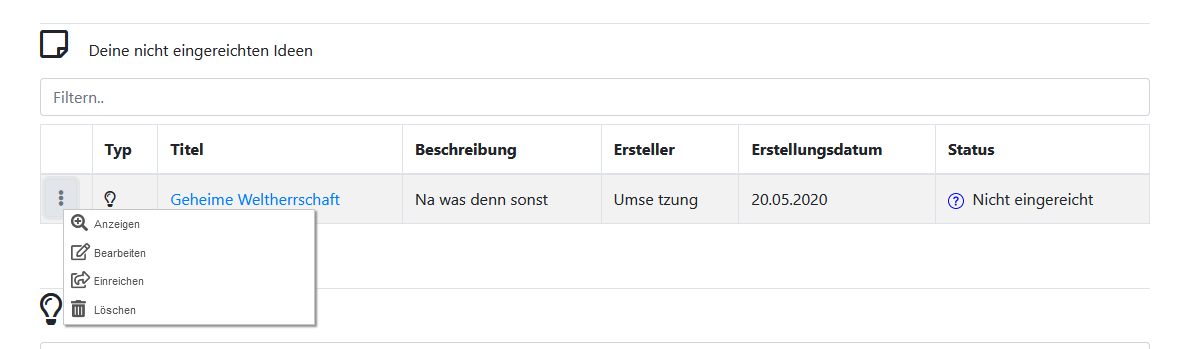
\includegraphics[width=1\textwidth]{img/rechtsklick-umsetzung.png}\\
    \source{Eigene Darstellung}
    \label{fig:rechtsklick}
\end{minipage}
\end{figure}

\begin{figure}[hbt]
\centering
\begin{minipage}[t]{1\textwidth}
    \caption{Dropdown Umsetzung}
    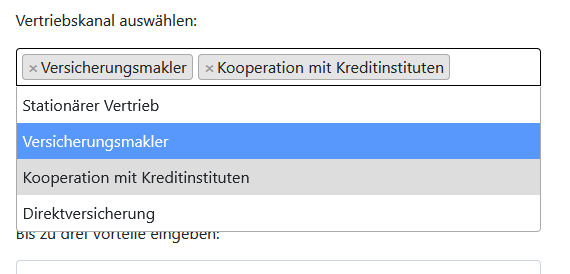
\includegraphics[width=0.5\textwidth]{img/dropdown-umsetzung.png}\\
    \source{Eigene Darstellung}
    \label{fig:dropdown}
\end{minipage}
\end{figure}

Hervorzuheben ist, dass gegenüber des Konzeptes in der Umsetzung\footnote{Siehe Anhang \ref{GUI-Umsetzung} auf S.\pageref{GUI-Umsetzung}} einige Elemente hinzugekommen sind. Die wichtigsten hierbei sind das bereits genannte Rechtsklick Menü (Siehe \cref{fig:rechtsklick}). Sowie intelligente Dropdown Menüs (Siehe \cref{fig:dropdown}).
Diese sollen dem Nutzer die Möglichkeit geben intuitiv die Anwendung zu bedienen und erweitern diese durch dynamische Menüs welche sich in die Oberfläche einpassen.
